% ==========================================
% Section 5: Normalization & Preprocessors (Slides 17-20)
% ==========================================

% Slide 17: Different Scales & Normalization
\begin{frame}{مقیاس‌های متفاوت ویژگی‌ها: نرمال‌سازی}
\begin{columns}[c]
  \begin{column}{0.60\textwidth}
    {\fontsize{9.5}{13.5}\selectfont
    \begin{itemize}
      \item \textbf{مرور: حساسیت شدید \lr{k-NN} به مقیاس ویژگی‌ها:}
      \begin{itemize}
        \item فاصله اقلیدسی سن و درآمد:\\
        {\footnotesize $D = \sqrt{(25-30)^2 + (70000-85000)^2} \approx 15000$}
        \item اثر تغییرات سن در برابر درآمد محو می‌شود!
      \end{itemize}
      \vspace{0.15cm}
      \item \textbf{راهکار: مقیاس‌بندی و استانداردسازی:}
      \begin{itemize}
        \item \textbf{\lr{StandardScaler:}} میانگین صفر و واریانس یک:\\
        {\footnotesize $z = \frac{x - \mu}{\sigma}$}
        \item \textbf{\lr{MinMaxScaler:}} نگاشت به بازه معین (معمولاً $[0, 1]$):\\
        {\footnotesize $X_{\text{norm}} = \frac{X - X_{\min}}{X_{\max} - X_{\min}}$}
      \end{itemize}
    \end{itemize}
    }
  \end{column}
  \begin{column}{0.38\textwidth}
    \centering
    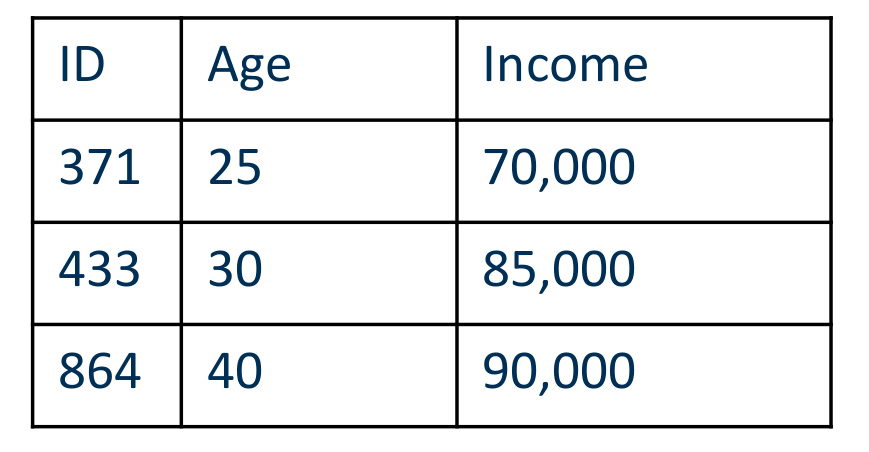
\includegraphics[width=\textwidth]{images/page_17_table.png}
  \end{column}
\end{columns}
\end{frame}

% Slide 18: Preprocessors Need to be Trained
\begin{frame}{پیش‌پردازشگرها نیز نیاز به آموزش دارند!}
\begin{columns}[c]
  \begin{column}{0.58\textwidth}
    \begin{itemize}
      \item \textbf{بسیاری از روش‌های پیش‌پردازش دارای حالت داخلی (\lr{Internal State}) هستند}
      \begin{itemize}
        \item به عنوان نمونه: میانگین و واریانس در \lr{StandardScaler}، یا کمینه و بیشینه در \lr{MinMaxScaler}.
      \end{itemize}
      \vspace{0.3cm}
      \item \textbf{هشدار مهم:}
      \begin{itemize}
        \item \alert{هرگز} پیش‌پردازش را روی کل مجموعه داده قبل از تقسیم‌بندی اعمال نکنید!
        \item این کار مصداق بارز \textbf{نشت اطلاعات (\lr{Data Leakage})} از داده‌های ارزیابی به آموزش است.
      \end{itemize}
    \end{itemize}
  \end{column}
  \begin{column}{0.40\textwidth}
    \centering
    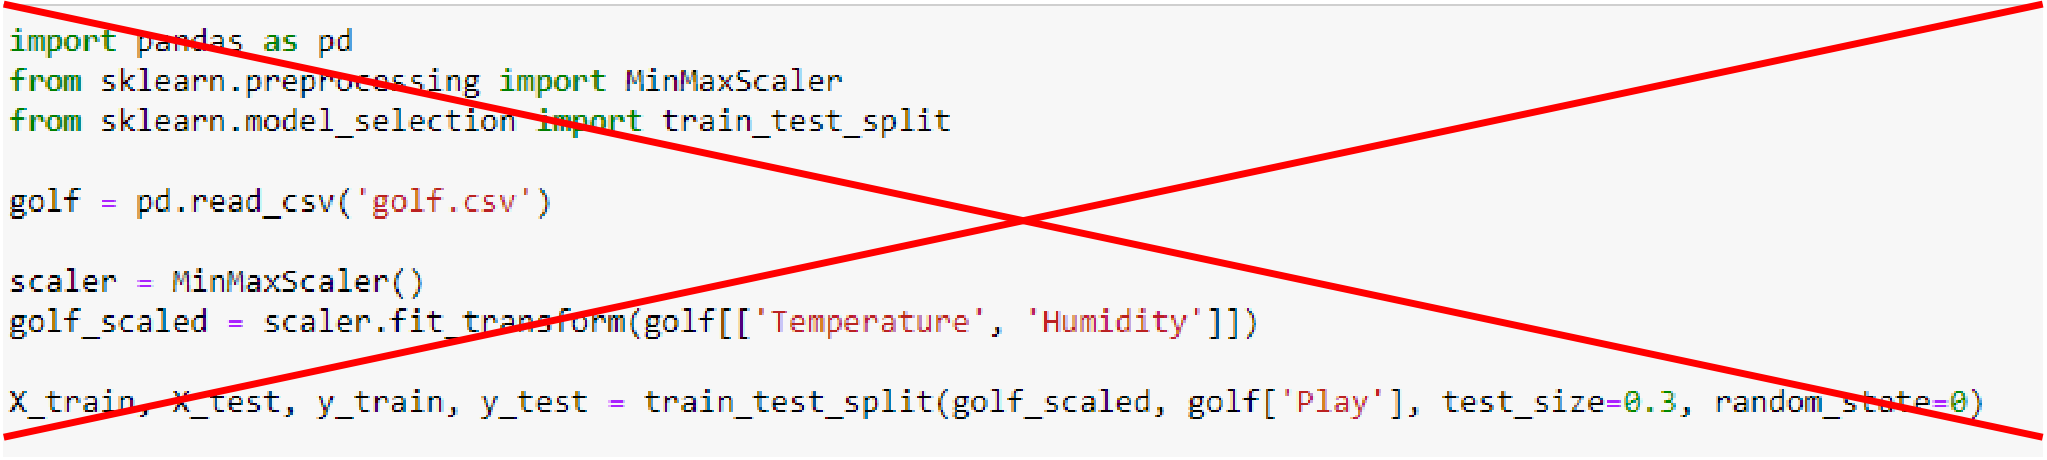
\includegraphics[width=\textwidth]{images/page_18_img_1.png}
  \end{column}
\end{columns}
\end{frame}

% Slide 19: Fit vs Transform
\begin{frame}{پیش‌پردازشگرها نیز نیاز به آموزش دارند (ادامه)}
\begin{columns}[c]
  \begin{column}{0.58\textwidth}
    \begin{itemize}
      \item \textbf{تفکیک فاز برازش (\lr{Fit}) و تبدیل (\lr{Transform})}
      \begin{itemize}
        \item تابع \lr{fit\_transform} منحصراً برای داده‌های آموزشی (\lr{Training Set}) استفاده می‌شود تا پارامترها را محاسبه و اعمال کند.
        \item تابع \lr{transform} برای داده‌های آزمون (\lr{Test Set}) استفاده می‌شود (با استفاده از پارامترهای آموخته‌شده از داده آموزش).
      \end{itemize}
      \vspace{0.3cm}
      \item این تفکیک ضامن ارزیابی واقع‌بینانه مدل در محیط واقعی است.
    \end{itemize}
  \end{column}
  \begin{column}{0.40\textwidth}
    \centering
    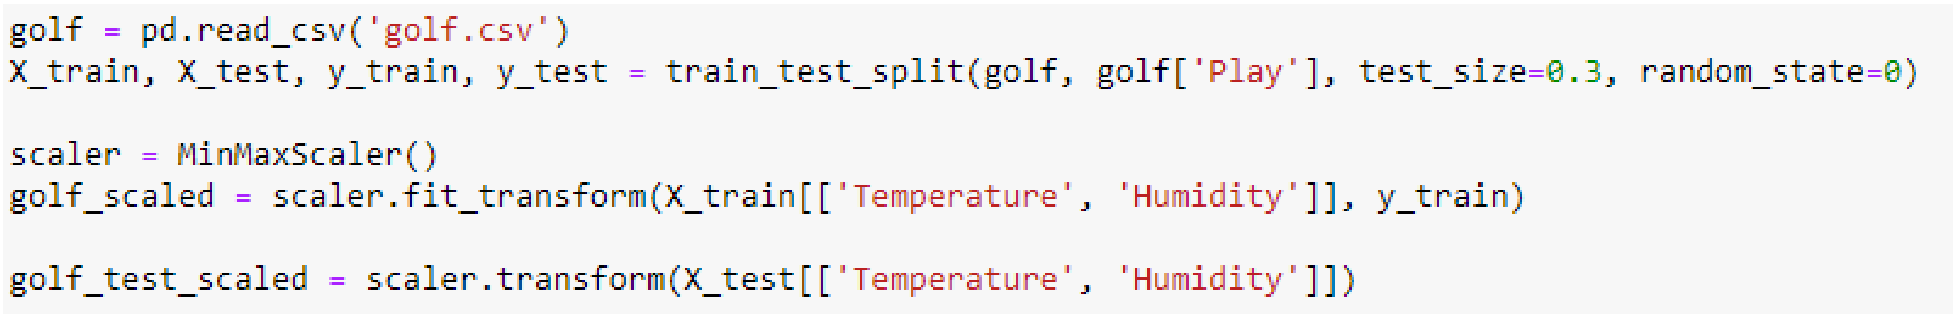
\includegraphics[width=\textwidth]{images/page_19_img_1.png}
  \end{column}
\end{columns}
\end{frame}

% Slide 20: Pipelines
\begin{frame}{ترکیب اجزای یادگیری ماشین: پایپ‌لاین‌ها}
\begin{columns}[c]
  \begin{column}{0.55\textwidth}
    \begin{itemize}
      \item \textbf{ساخت زنجیره پردازشی منظم با \lr{Pipeline}}
      \begin{itemize}
        \item تجمیع پیش‌پردازشگرها و مدل تخمین‌زننده در یک شیء واحد.
        \item جلوگیری خودکار از نشت داده در اعتبارسنجی متقاطع (\lr{Cross-Validation}).
      \end{itemize}
      \vspace{0.2cm}
      \item \textbf{اعمال تبدیل‌های مجزا بر ستون‌های مختلف:}
      \begin{itemize}
        \item استفاده از \lr{ColumnTransformer} برای اعمال پایپ‌لاین‌های متفاوت بر ویژگی‌های عددی و متنی/دسته‌ای.
      \end{itemize}
    \end{itemize}
  \end{column}
  \begin{column}{0.43\textwidth}
    \centering
    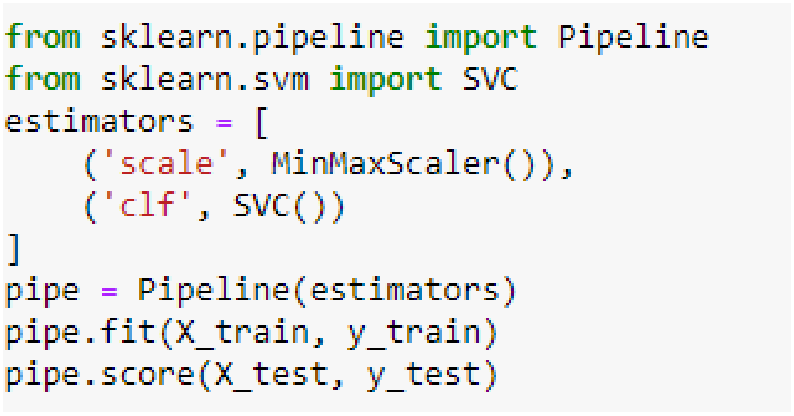
\includegraphics[width=\textwidth]{images/page_20_img_1.png}\\[6pt]
    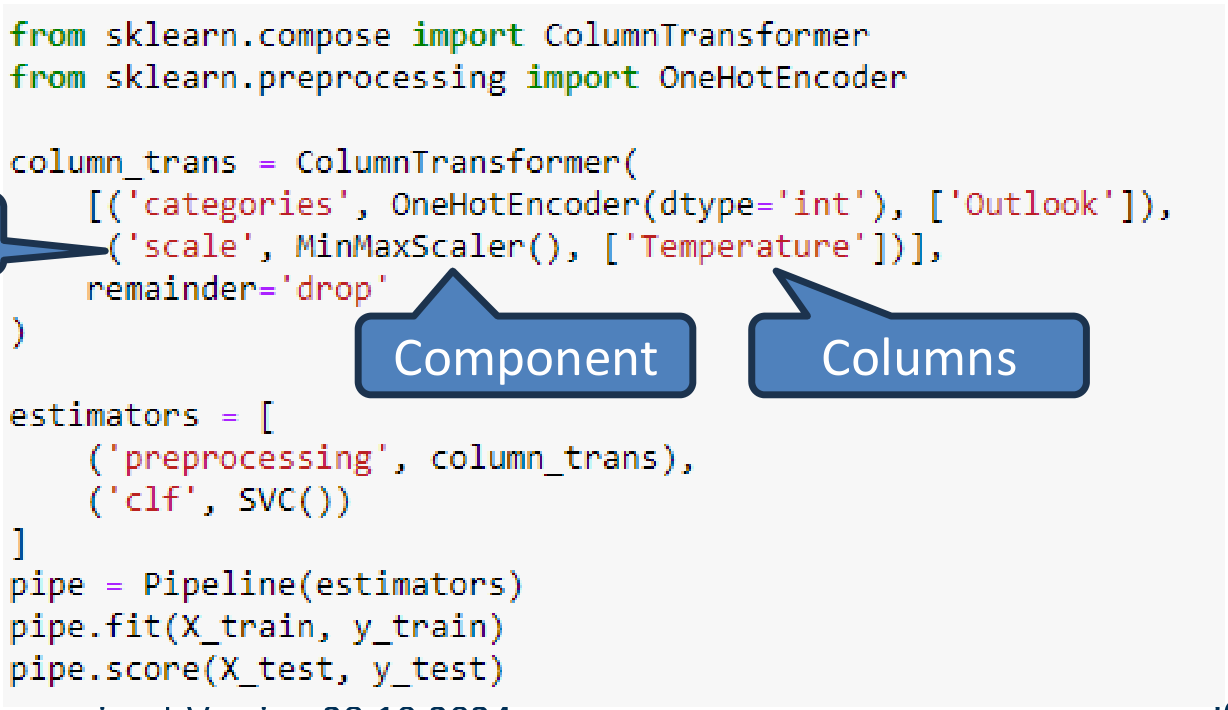
\includegraphics[width=\textwidth]{images/page_20_img_2.png}
  \end{column}
\end{columns}
\end{frame}
